\documentclass[12pt]{article}
\usepackage{sydewkrpt}
\usepackage{amsmath}

%%%%%%%%%%%%%%%%%%%%%%%%%%%%
%%%    Begin Document    %%%
%%%%%%%%%%%%%%%%%%%%%%%%%%%%
\begin{document}
\pagenumbering{roman}

\waterlootitle{ME 597: Assignment 1}{

  }{
  Sarah Elliott
  Leigh Pauls\\
  \today
  }

\newpage
\singlespacing
\pagenumbering{arabic}
\section{Bicycle Model}
\setlength{\parindent}{1cm}

For the bicycle model, we basically need to find the \textit{$x_t$} and \textit{$y_t$} for each time step. We add Guassian noise to the position with \textit{$\sigma_{xy}$ = 0.02 m}.
\begin{equation}
\onehalfspacing
\centering
\emph{ $x_t$ = $x_{t-1}$ + $d_t$*cos($\mu_{heading}$) + N(0, $\sigma_{xy}$)}
\end{equation}
\begin{equation}
\onehalfspacing
\centering
\emph{ $y_t$ = $y_{t-1}$ + $d_t$*sin($\mu_{heading}$) + N(0, $\sigma_{xy}$)}
\end{equation}
 Within that we get \textit{$d_t$}, which is the distance traveled since the last time step by multiplying the speed \textit{v = 3 m/s} by the time step  \textit{dt = 0.1 s}: 
\begin{equation}
\onehalfspacing
\centering
\emph{ $d_t$ =  v*dt}
\end{equation}
We now need to get the heading. The heading, \textit{$h_t$}, is shown below. We add Guassian noise to the angle calculated with \textit{$\sigma_\theta$ = 1$^\circ$}.
\begin{equation}
\onehalfspacing
\centering
\emph{ $h_t$ = $h_{t-1}$ + dheading*dt + N(0, $\sigma_\theta$)*dt}
\end{equation}
The change in heading, \textit{dheading}, for the time step is found by:
\begin{equation}
\onehalfspacing
\centering
\emph{ dheading = v*tan($\delta$)}
\end{equation}
The average heading, \textit{$\mu_{heading}$}, used in the first equation is: 
\begin{equation}
\onehalfspacing
\centering
\emph{ $\mu_{heading}$ = $\frac{h_t + h_{t-1}}{2}$}
\end{equation}
The above equations all rely on \textit{$\delta$}. The instructions give a max steering angle of +/-30$^\circ$.
\[ 
      \delta = 
      \begin{cases} 
      30^\circ & t > 40\\
      10 - t & t < 40
   \end{cases}
\]
The resulting path for a start position of (0,0) and heading of 0$^\circ$ is shown below:
\begin{figure}[ht]
\hspace{0.5cm}
\centering
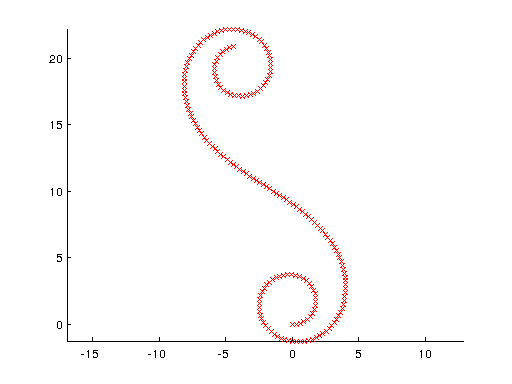
\includegraphics[scale=0.5]{Pictures/bikemodel.png}
\end{figure}

\newpage
\singlespacing
\section{Carrot Planner}
\setlength{\parindent}{1cm}

The robot needs to track a rectangular path. The path \textit{A} is defined by 4 points.
\begin{equation}
\onehalfspacing
\centering
\emph{P =\textnormal{\lbrack} $p_1 p_2 p_3 p_4$ \textnormal{\rbrack} }
\end{equation}
To find the closest point on the path you need to know which part of the path is closest. We can imagine the path as having 4 segments, one for each side of the rectangle. Segment \textit{S($p_n, p_{n+1}$)} is the segment with start and end points at \textit{$p_n$} and \textit{$p_{n+1}$} respectively, where \textit{n = 1, 2, 3}. For each \textit{S}, we need to find the closest point on that segment. Then we will compare the closest points on each segment to see which of the segments is the closest overall. 

Let \textit{$p_{cur}$} be the current point. Let \textit{$r_{p_n/p_{n+1}}$} be the distance between those two points. This notation is extended to all other distances between points. The distance calculation is fairly trivial and not included in this report. Let's define the distance from the first waypoint, \textit{$p_n$}, of the current segment to the closest point on the line as \textit{$d_c$}. 
\begin{equation}
\onehalfspacing
\centering
\emph{$d_c$ = $r_{p_{cur}/p_n}$ * $\frac{r_{p_{n+1}/p_{cur}}^2 -  r_{p_n/p_{cur}}^2 - r_{p_{n+1}/p_n}^2}{-2*r_{p_n/p_cur}*r_{p_{n+1}/p_n}}$ }
%\frac{$r_{p_{cur}/p_{n+1}}^2$ -  $r_{p_{cur}/p_n}^2$ - $r_{p_n/p_{n+1}}^2$}{-2*$r_{p_cur/p_n}$*$r_{p_n/p_{n+1}}$}}
\end{equation}
The figure below shows an example of \textit{$d_c$}. Other point configurations are possible. 
\begin{figure}[ht]
\hspace{0.5cm}
\centering
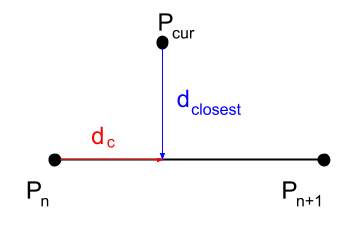
\includegraphics[scale=0.5]{Pictures/points_1.png}
\end{figure}
To find the closest point on the line we have to consider a number of cases. If the points are oriented as above, finding the closest point is fairly straight forward. You just add  \textit{$d_c$} to the location of \textit{$p_n$}. However, what if  \textit{$p_{cur}$} is closest to the top edge of the rectangle and moving counterclockwise? This would mean you need to subtract  \textit{$d_c$} from the location of \textit{$p_n$}. Other cases include if \textit{$d_c$} is negative or greater than \textit{$r_{p_{n+1}/p_n}$}; for example if \textit{$p_{cur}$} is outside the rectangle. To take all these situations into account:
\[ 
      p_{closest} = 
      \begin{cases} 
      p_n & d_c < 0\\
      p_n + d_c * \frac{p_{n+1} = p_n}{r_{p_{n+1}/p_n}} & r_{p_{n+1}/p_n} > d_c > 0 \\
      p_{n+1} & d_c > r_{p_{n+1}/p_n}\\
   \end{cases}
\]
This is repeated for every line segment and the line segment where the distance between $p_{cur}$ and $p_{closest}$ is chosen. Then that $p_{closest}$ is the overall closest point. To set the actual desired carrot position, check how mush distance is left on the line until the next waypoint. If the distance left is less than \textit{r =1} then the next waypoint is the carrot position. Otherwise, it computes the carrot position as follows:
\[ 
      p_{carrot} = 
      \begin{cases} 
      p_{n+1} & r > r_{p_{n+1}/p_{closest}}\\
      p_{closest} + r * \frac{p_{n+1} + p_{closest}}{r_{p_{n+1}/p_{closest}}} & r < r_{p_{n+1}/p_{closest}} \\
   \end{cases}
\]
To steer towards that position we find the the vector distance between the current position and carrot position, \textit{$r_{p_{carrot}/p_{current}}$}. Then the desired heading is:
 \begin{equation}
\onehalfspacing
\centering
\emph{$h_{desired}$ = arctan($\frac{r_{p_{carrot}/p_{current}x}}{r_{p_{carrot}/p_{current}y}}$)}
\end{equation}
\[ 
      h_{error} = 
      \begin{cases} 
      h_{error} - 2*\pi & h_{error} > \pi \\
      (h_{desired} - h_{t-1}) \% 2*\pi & h_{error} < \pi
   \end{cases}
\]
We make the steering angle using proportional control (in this case we multiply our steering angle error by 1 to get a new steering angle).
\begin{equation}
\onehalfspacing
\centering
\emph{$\delta$= 1 * $h_{error}$ }
\end{equation}
Then we just feed that steering angle into the bike model from the previous question.
The resulting plot of the robot driving around the rectangle is shown below. It starts with an abitrary position at (10, 1) with a heading of 90$^\circ$.
\begin{figure}[ht]
\hspace{0.5cm}
\centering
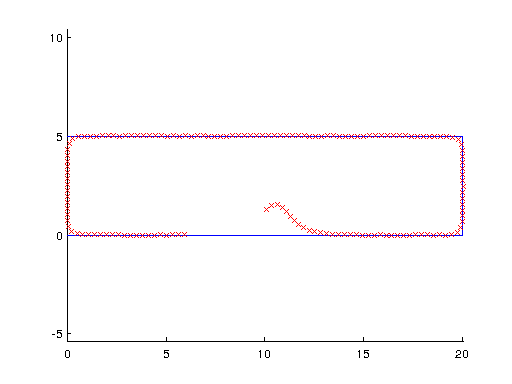
\includegraphics[scale=0.5]{Pictures/carrot.png}
\end{figure}


 




\end{document}
